\documentclass[11pt]{report}
\usepackage{StyleSheets/main}
\begin{document}

\chapter{Detailed Design}\label{ch:detailed-design}
This section will give a detailed design of the vehicle, its components, and special design features. It is to serve as a breakdown of the vehicle's structure, detailing every part of the vehicle. In this section, the vehicle's special design features, a decomposition of the structure, circuitry of the vehicle, and the software architecture will be discussed and detailed. 

\section{Body of the Vehicle}

\subsection{General Structure}
The base of this vehicle's structure is a singular 1116 Series Grid Plate (to be referred to as bottom grid plate). This grid plate has a  17 x 29 hole configuration, with each hole being $\SI{4}{\milli\meter}$ in diameter. The size of the bottom grid plate is 136 x $\SI{232}{\milli\meter}$, and is $\SI{2.5}{\milli\meter}$ thick. This grid plate serves as a strong and sturdy base for the structure of the vehicle, and is at the core of all connections made. One of the ends of this bottom grid plate will be referred to as the front, which mounts the ultrasonic sensors, gripper, and color sensors. At the back end of the vehicle were 2 U-shaped connecting pieces, which served as a cover for the battery. These U-shaped pieces were placed on both sides of the vehicle, and the $\SI{12}{\volt}$ battery was placed with its full length being perpendicular to the length of the grid plate. On top of this U-shaped connector, was placed another grid plate. This grid plate was of the same specification as the original grid plate, although it was also placed perpendicular to the length of the bottom grid plate, and in the same orientation as the battery. Two breadboards were placed on this top grid plate. One breadboard served as a place to house the Teensy 4.1 microcontroller, and the other was used for power distribution around the circuit as well as an \gls{LED} to indicate the state of the system. The breadboards and Teensy 4.1 microcontrollers are discussed in \cref{sec:wiring,sec:breadboard-and-pins}.

\par The gripper was placed on the front of the bottom grid plate. The structure of the gripper is discussed in \cref{sec:gripper}. On either side of the gripper a mount was placed for the ultrasonic and color sensors. These sensor mounts allowed for the vehicle to complete the tasks of color recognition, obstacle avoidance, and line following. Underneath the bottom grid plate sat the motor controllers which were placed with spacers between the plate and the controllers to avoid unwanted interruptions in the circuit. 2 motor controllers were used, each powering 2 of the 4 motors used. The 4 motors, attached to the vehicle using 2 side clamping mounts, were placed on each side of the vehicle, in the middle of each length. These mounts were placed underneath the bottom grid plate, and each had a brushed \gls{DC} 26 \gls{RPM} motor attached. To the ends of these motors, was attached an omni wheel, which allowed the vehicle to move in any direction in a crab-walk configuration. Over the front wheel and underneath the gripper was placed a sensor mount, which allowed for the attachment of an additional ultrasonic sensor in front of the vehicle, which was in the center and further forward than the other sensors. 

\subsection{Wheels}
The system utilized a crab-walk design, having a wheel on either side of the vehicle as well as the front and back. This configuration allowed for the vehicle to have 2 degrees of freedom in movement, with the side wheels allowing for forward and backwards movement and the back and front wheels allowing for side to side movement. The wheels, which were chosen to be omni-wheels, allowed for the smooth movement of the vehicle in every direction. This design allowed for higher speeds in every direction, with each direction of movement allowing 2 motors to push the necessary wheels. 
\par During testing, the issue of the wheels slipping during sideways movement of the vehicle came up. The weight was unevenly distributed throughout the robot, causing it to not allow the side wheels to both be in contact with the ground at a time. The solution for this problem was to introduce a suspension system, which allowed the motor mounts to bend outwards allowing the vehicle to have all wheels in contact. On the right side of the vehicle, a spring was placed along with a series of washers to the motor mounts connection points with the grid plate. This allowed the connection to be looser and have more flexibility. On the other side of the vehicle, the bottom of the motor mount included springs, which pulled the wheel closer to the vehicle but allowed for more flexibility. The introduction of the suspension system allowed the robot to move in every direction effectively. 

\subsection{Motors}
The motors attached to these wheels were 26 \gls{RPM} \gls{DC} motors. These motors provided the vehicle with the necessary speed to complete the tasks in a faster time. The side 26 \gls{RPM} motors were modified using 116 \gls{RPM} motor’s gearboxes, which gave the vehicle additional speed in the forward and backward directions. 

\subsection{Battery}
The battery used in this vehicle was a $\SI{12}{\volt}$ battery with an on and off switch, a charging port, and a connection port for wires to be connected to the rest of the circuit. All of the vehicle’s power came from this battery. The placement of the battery allowed for easy changing between on and off during testing, which simplified the process massively. The battery being situated at the back of the vehicle allowed for the weight to be distributed evenly throughout the vehicle, as it balanced the weight of the gripper on the front. The wiring of the battery to the rest of the circuit will be discussed in later sections. 

\subsection{3-D Printed sensor mounts}
\subsubsection{Ultrasonic Sensor and Color Sensor Mounts}
The ultrasonic sensors and color sensors were placed on the 3D printed sensor mounts. The design is shown in Figure B.12. These mounts were attached to the bottom grid plate on either side of the vehicle’s front wheel. The side sensor mounts were designed to house the ultrasonic sensors in a position where they would sense further outwards than the furthest edge of the wheel to avoid the vehicle hitting the obstacles during the tests. The ultrasonic sensors were placed in a forward facing position, while the color sensors were attached facing towards the floor for color recognition. The color sensors were housed by a curtain as a part of the sensor mounts to avoid external light messing with the color sensing ability.
\subsubsection{Front-Central Ultrasonic Sensor Mount}
The middle ultrasonic sensor mount had a design to which it would attach to the top of the bottom grid plate and curve over the top of the front wheel. This curve was such that it would not interfere with the front wheel, and there was sufficient space for the attachment of wires to the ultrasonic sensor without interference. This design allowed for the central front facing ultrasonic sensor to be further forward than the rest of the vehicle, and allowed for the vehicle to sense the platform on which the box is located for the pickup and placement test. The front-central ultrasonic sensor mount can be seen in Figure B.8.

\subsubsection{Lower Infrared Sensor and Color Sensor Mount}
The vehicle’s \gls{IR}/\gls{RGB} sensor mount was located beneath the vehicle, and allowed for the sensors to be as close to the ground as possible for accurate centering about the target-line. The mount was attached to the motor mount of the front wheel, and the \gls{IR} sensor was located right underneath this mount. The sensor mount also acted as an electrical spacer to avoid unwanted contact with metals and the \gls{IR} sensor. The lower \gls{IR} sensor mount can be seen in Figure B.9. 

\section{Gripper}\label{sec:gripper}
\subsection{Gripper Arm}
The arm of the gripper was made up of many plates and connecting pieces. Firstly, a U-shaped connection plate was attached to the front of the vehicle, occupying the same holes in the grid plate as the front-central ultrasonic sensor and the front wheel. This U-shaped plate raised the gripper above the vehicle and allowed for the gripper to not come in contact with the wheel. Attached to this is another U-shaped plate of the same shape, and inside this is the servo motor which controls the movement of the gripper arm. This servo motor allows the gripper to move with one degree of freedom, and controls the angle at which the gripper is facing. The servo motor is attached to the rest of the arm using a metal rod which is attached to a longer plate. This longer plate extends the length of the gripper arm, and allows the hand of the gripper to reach the box in the pickup and placement system. The end of this arm plate marks the end of the gripper arm before the hand system starts, with a U-shaped grid plate attached to the end of the arm. 
\subsection{Gripper Hand}
The gripper hand is made up from multiple smaller components. Attached to the gripper arm is the claws of the gripper, which are 2 pieces of plastic with extensions to reach the box. These extensions are controlled using a gear system which is connected to another servo motor, which has the use of controlling the opening and closing of the gripper hand. The ends of the extensions have 3D printed mounts attached, which will be detailed shortly. 
\subsection{Gripper Sensor Mounts and Sensors}
The sensors for the gripper hand were attached to the claw of the gripper using 3D printed sensor mounts. The sensors on the gripper were used to determine box size, box color, and height of the gripper above the platform. 
\subsubsection{Left Gripper Sensor Mount and Sensors}
The left sensor mount was used as an extension to the gripper claw which allowed for the vehicle to more effectively grab the box. Within the extension was placed the color sensor, which had the task of sensing whether the box was blue or red. The left gripper sensor mount can be seen in Figure B.11.
\subsubsection{Right Gripper Sensor Mount and Sensors}
The sensor mount on the right hand side of the vehicle’s gripper had the purpose of allowing the box to be better grabbed as it was an extension of the claw, and also served as a place for an infrared sensor and a button. The infrared sensor allowed the robot to know when it was near the platform and could drop the box. The button had the purpose of letting the robot know which size box was being picked up. The time from when the gripper started closing and when the button was pressed was measured and the robot used this information to determine the box size. The right gripper sensor mount can be seen in Figure B.10.

\subsection{Added Component Cost}
A total of \$1.65 of the provided \$25 budget were used for both prototyping and final iterations of the aforementioned sensor mounts, and another \$4.99 for the \gls{IR} array. 3D-prints were done efficiently by sending multiple of the same design to print simultaneously to avoid failures that would further delay our design and testing processes. A complete breakdown of the cost, including both the 3D-printing and \gls{IR} array, can be found in \cref{ap:diagrams}.

\section{Breadboards and Pins}\label{sec:breadboard-and-pins}
\subsection{Teensy 4.1 Microcontroller}
Placed on one breadboard was the Teensy 4.1 Microcontroller. The microcontroller was an integral part of this system which allowed a computer to communicate with the robots movements and features using code which was implemented to the system. The Teensy 4.1 microcontroller has a series of pins which connect to the color sensors, the ultrasonic sensors, the infrared sensors, the motors (through the motor controllers), and the servo motors. The Teensy 4.1 pinout map can be seen in Figure B.14. 
\par Each pin in the Teensy 4.1 had a wire connecting it to the required part of the robot, in a complicated wire network which is discussed shortly. 

\subsection{DC-DC Converters}
The second breadboard used contained two \gls{DC}-\gls{DC} converters (buck converters). These were used to bring the voltage from the $\SI{12}{\volt}$ battery down to a more usable voltage for the system, and was controlled using a potentiometer built into the buck converter. 
\par One DC-DC converter was used to step down the $\SI{12}{\volt}$ from the battery to $\SI{7.4}{\volt}$ for the use of the motors which drive the vehicle. This voltage allowed the motors to operate at maximum capacity. The other converter was used to power the Teensy 4.1, stepping the voltage down to $\SI{5}{\volt}$.

\subsection{LED System}
The \gls{LED} system on the breadboard represented a system to show whether the battery was turned on or not. If the battery was on, the \gls{LED} would shine and if not, it would turn off. This helped know whether the system was active or not. The \gls{LED} was connected to the system using the voltage from the \gls{DC}-\gls{DC} converters and a resistor in series with the \gls{LED}.

\section{Wiring}\label{sec:wiring}
\subsection{Sensors}
In testing, it became clear that wiring would be an important factor for the simplicity of the system. The final robot had a simplified wiring system for the sensors. Each sensor has a set of pins to which connections need to be made. The color sensor pin map can be seen in Figure B.15. 
\par At the front of the robot, the sensor mounts allowed for the wires of the ultrasonic and color sensor wiring to be greatly simplified and to not interrupt any other use of the vehicle. The wires and wire extensions connected the sensors to the Teensy 4.1 microcontroller in their respective ports.

\subsection{Gripper}
The wiring on the gripper was important as it is a moving piece and could mess up the system if done incorrectly. The gripper, the servo motors, and the gripper sensors all connected back to the Teensy microcontroller. 

\subsection{Motor Controllers}
The two motor controllers situated underneath the lower grid plate bot controlled two motors each. This was done by making the motors closest to the controller the connection. The wires were soldered together at a connection point and then connected to the Teensy and buck converter. 

\subsection{Simplification and Neatness Strategy}
Making sure the wiring in the system was neat and usable was a very important part of this robot. The wires were held together using cable ties, and were attached to the grid plate using the same method. This ensured that all wires from a particular sensor were held together and there were no loose wires. The sensor mounts allowed for additional simplification, as well as the soldering of the motor and motor controller wires. 
\par Each wire corresponded with a particular color in accordance to \cref{fig:Pinoutmap}, which helped maintain the simplicity of the system and allowed for knowing what comes where. 

\subsection{Circuit Diagram}
The circuit diagram for this system is available in the diagrams section, and is seen in \cref{fig:CircuitDiagram}. This details the connections between the microcontroller and the color sensors, ultrasonic sensors, \gls{IR} array, gripper servo motors, and motors. This circuit diagram details where the power comes from in each component.

\section{Code}
 The code was designed as a modular system with each sensor having it's own class, allowing for an incredibly flexible and readable system. The code is found in \cref{ap:code}.

\subsection{Color Sensors}
The basic use of the color sensors was for the robot to recognize certain colors and make decisions based on that recognition. The code can be found in \cref{lst:colorsensor-h}. The color sensors on the mounts under the base of the vehicle allowed the vehicle to sense colors of lines. For the obstacle avoidance test, the vehicle used these color sensors to recognize the end of the obstacle course which was represented by a white line. Once the vehicle saw this white line, a delay was implemented into the code and the vehicle would come to a stop. In the line following test, the vehicle would use the color sensors to recognize the green lines at the starting and ending point of the course. The color sensors were also used when the vehicle was turning around, as it used them to recognize when it was on and off the line. The color sensors at the bottom of the vehicle were also used to recognize the edge of the course for both tests, stopping when the sensors recognized the white lines at the sides.

\par The color sensor on the gripper was important for the robot to recognize which path it would follow based on which color box it picked up. If the gripper sensed that the box was blue, the robot would then follow the blue line, and if the gripper sensed that it was red, it would follow the red line. Additionally, the gripper color sensor was only calibrated with red and blue colors, as those were the only colors that the box could be.

\par Due to the incredibly reflective surface of the tarp \& the tape colors, it was difficult to reliably sense the colors. Because of this issue, a bespoke method of determining the color was created. First, the colors were represented as points in a 3D space, with the red frequency being the $x$-axis, green being the $y$-axis, and blue being the $z$-axis. Then, many calibration points were taken with each of the sensors. The visualization of these calibration points can be found in \cref{sc:color-sensor-points}.

\par To determine what color the robot actually saw, the robot took the current RGB values that were read and compared them to a database of calibration points, (found in \cref{lst:initialization-h}), determining which calibration point was the closest in euclidean distance. This is visualized below in \cref{fig:color-calibration-distance-example}.

\par However, even with over a thousand calibration points, the reflectivity was so high that additional measures had to be put into place to make certain the colors read were correct. Instead just using the color corresponding to the minimum distance calibration point, a moving average was taken as well. Given a moving average window, if the majority of the previously read points were that color, only then would it return with that color. This allows for a smoothing to the color reading, so if one or two erroneous readings come from the reflectivity, they will be ignored due to the bulk of other data.  Each time the color sensor wasn't being read continuously the history had to be reset. For example, if the color history was filled up with black, and then the robot was moved to a different section over red, then the color sensors turned back on, the colors read initially would be black as the history was already filled.

\documentclass[12pt]{report}
\usepackage{GraphDefinitions}

\begin{document}

\def\grayopacity{0.055}
\def\ballsize{3pt} % Change the size of the balls
\def\seencolor{orange}
\def\seenx{543}
\def\seeny{340}
\def\seenz{500}
\def\calix{574}
\def\caliy{271}
\def\caliz{435}
\def\calicolor{blue}
\def\maxy{750}
\def\maxx{825}
\def\shadowopacity{0.4}
            
\begin{figure}[H]
    \centering
    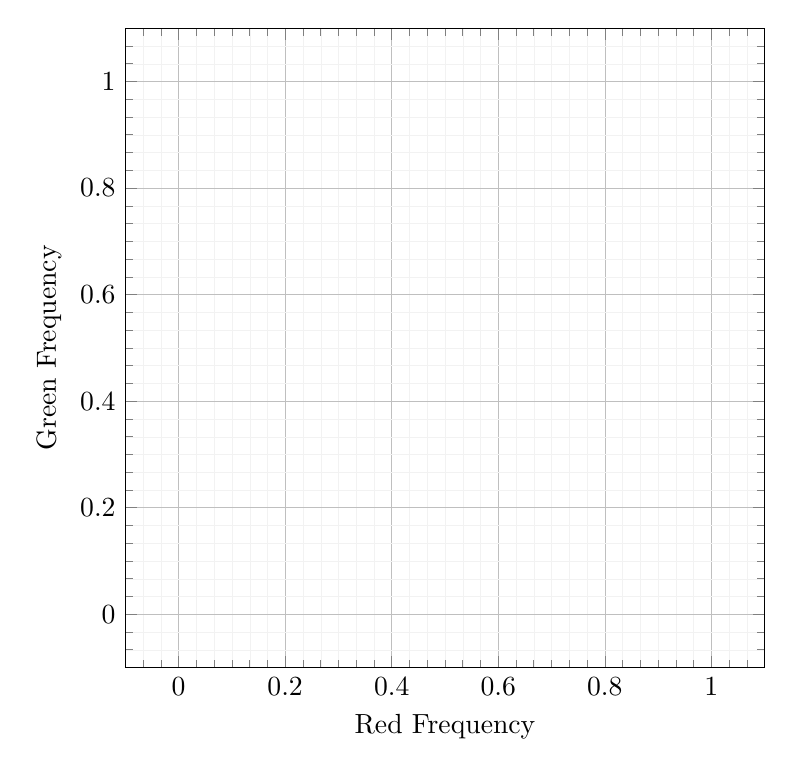
\begin{tikzpicture}
        \begin{axis}[
            xlabel={Red Frequency},
            ylabel={Green Frequency},
            zlabel={Blue Frequency},
            xlabel style={sloped like x axis}, % Make x label follow the x axis
            ylabel style={sloped like y axis}, % Make y label follow the y axis
            zlabel style={sloped}, % Make z label follow the z axis or make it vertical
            legend pos=north west,
            grid=both,
            grid style={line width=.1pt, draw=gray!10},
            major grid style={line width=.2pt,draw=gray!50},
            minor tick num=5,
            width=0.8\textwidth,
            height=0.8\textwidth,
            view={-80}{45}, % Adjust the view angle for better visualization
        ]
        \IfFileExists{code/output_data/color_sensor_calibration/rightColor.csv}{

            % SEEN point
            \addplot3[only marks, ball color=\seencolor, mark=ball, mark size = \ballsize*1.3, draw opacity = 0] coordinates {(\seenx, \seeny, \seenz)};
            \addlegendentry{Frequencies Read by Sensor}

            % CALIBRATION point
            \addlegendentry{Closest Calibration Point \& Used Color}
            \addplot3[only marks, ball color=blue, mark=ball, mark size = \ballsize*1.3, draw opacity = 1, draw= \seencolor, line width = 0.5mm] coordinates {(\calix, \caliy, \caliz)};

            % Line between the two
            \addplot3[ no marks,thick, line width=0.5mm, color=\seencolor, opacity = 1, -latex] coordinates {(\seenx, \seeny, \seenz) (\calix, \caliy, \caliz)};

            % Determine opacity based on sensor

            \addplot3[
                only marks,
                scatter,
                scatter/classes={
                    RED={mark=ball,ball color= red, draw opacity=0, mark size = 0},
                    BLUE={mark=ball,ball color= blue, draw opacity=0, mark size = \ballsize},
                    GREEN={mark=ball,ball color= green, draw opacity=0, mark size = 0},
                    WHITE={mark=ball,ball color= white, draw opacity=0, mark size = 0},
                    BLACK={mark=ball,ball color= black, draw opacity=0, mark size = \ballsize},
                    YELLOW={mark=ball,ball color= yellow, draw opacity=0, mark size = 0}
                },
                scatter src=explicit symbolic,
            ] table[
                x=Red_Freq,
                y=Green_Freq,
                z=Blue_Freq,
                meta = Color,
                col sep=comma,
            ] {code/output_data/color_sensor_calibration/rightColor.csv};

            % Wall histogram on the left
            \addplot3[
                only marks,
                scatter,
                scatter/classes={
                    RED={mark=*,fill=gray, fill opacity=0, draw opacity=0},
                    BLUE={mark=*,fill=gray, fill opacity=\grayopacity, draw opacity=0},
                    GREEN={mark=*,fill=gray, fill opacity=0, draw opacity=0},
                    WHITE={mark=*,fill=gray, fill opacity=0, draw opacity=0},
                    BLACK={mark=*,fill=gray, fill opacity=\grayopacity, draw opacity=0},
                    YELLOW={mark=*,fill=gray, fill opacity=0, draw opacity=0}
                },
                scatter src=explicit symbolic,
            ] table[
                x = Red_Freq,  % This sets the x-coordinate to 0
                y expr = 800,  % This sets the y-coordinate to 0
                z= Blue_Freq,
                meta = Color,
                col sep=comma,
            ] {code/output_data/color_sensor_calibration/rightColor.csv};

            % Wall histogram on the right
            \addplot3[
                only marks,
                scatter,
                scatter/classes={
                    RED={mark=*,fill=gray, fill opacity=0, draw opacity=0},
                    BLUE={mark=*,fill=gray, fill opacity=\grayopacity, draw opacity=0},
                    GREEN={mark=*,fill=gray, fill opacity=0, draw opacity=0},
                    WHITE={mark=*,fill=gray, fill opacity=0, draw opacity=0},
                    BLACK={mark=*,fill=gray, fill opacity=\grayopacity, draw opacity=0},
                    YELLOW={mark=*,fill=gray, fill opacity=0, draw opacity=0}
                },
                scatter src=explicit symbolic,
            ] table[
                x expr = 750,  % This sets the x-coordinate to 0
                y = Green_Freq,  % This sets the y-coordinate to the back wall
                z= Blue_Freq,
                meta = Color,
                col sep=comma,
            ] {code/output_data/color_sensor_calibration/rightColor.csv};

            % Floor histogram
            \addplot3[
                only marks,
                scatter,
                scatter/classes={
                    RED={mark=*,fill=gray, fill opacity=0, draw opacity=0},
                    BLUE={mark=*,fill=gray, fill opacity=\grayopacity, draw opacity=0},
                    GREEN={mark=*,fill=gray, fill opacity=0, draw opacity=0},
                    WHITE={mark=*,fill=gray, fill opacity=0, draw opacity=0},
                    BLACK={mark=*,fill=gray, fill opacity=\grayopacity, draw opacity=0},
                    YELLOW={mark=*,fill=gray, fill opacity=0, draw opacity=0}
                },
                scatter src=explicit symbolic,
            ] table[
                x = Red_Freq,
                y = Green_Freq,
                z expr = 0,
                meta = Color,
                col sep=comma,
            ] {code/output_data/color_sensor_calibration/rightColor.csv};

            
        }{}
        \end{axis}
    \end{tikzpicture}
    \caption{Visual representation of color matching algorithm.\protect\footnotemark}
    \label{fig:color-calibration-distance-example}
\end{figure}
\footnotetext{The orange dot is the seen color by the sensor, and the nearest calibration point is blue, thus the color seen is set to blue.}

\end{document}

\subsection{Ultrasonic Sensors}
The code is found in \cref{lst:ultrasonic-h}. The 3 ultrasonic sensors had 2 different uses. The outer ultrasonic sensors were used in the obstacle avoidance testing, allowing for the vehicle to sense when an obstacle was blocking the vehicle, and become parallel. The sensor mounts allowed for these ultrasonic sensors to be wider than the wheels allowing the vehicle to not hit the obstacles on passing, due to the nature of how the sensors project. If the ultrasonic sensors sensed something was in the way, the vehicle was programmed to move sideways until it found a way through. 

\par The central ultrasonic sensor was used to recognize the distance from the vehicle to the platform for the box pickup and placement. This allowed the vehicle to get to the best possible distance for the gripper to grab the box effectively and allow the button on the box to be pressed.

\subsection{IR Array sensor}
The \gls{IR} array sensor was used to determine the ``centeredness'' on a line. Since the \gls{IR} array was placed in the middle of the vehicle, (seen in \cref{fig:underside}), if the \gls{IR} array had it's middle sensors activated, the vehicle was correctly following the line. If the sensors on the right of the \gls{IR} array were activated, the vehicle would correct and move to the right. If the sensors on the left of the \gls{IR} array were activated, the vehicle would correct and move to the left. This was implemented as the best form of line following due to the inconsistencies of the color sensors as a line following mechanism. Additionally, each tape color had a slightly different value returned from each sensor, and thus calibration points were taken for each color individually, seen in \cref{ir-calibration-data}.

\par The algorithm to determine the ``centerdness'' of the sensor based on which sensors on the array were lit up was somewhat involved. The \gls{IR} sensors would return either a $1$ or a $0$ depending on if they sensed a line or not. This was then weighted based on their position on the array, with the sensors on the edges of the array receiving a higher weighting than the center. The left sensors were weighted negative and the right sensors were weighted positive. Additionally, it was designed that if just the leftmost sensor was activated, it would be $-1$, and if just the rightmost sensor was activated, the error would return $+1$. The left sensors had their value averaged and the right sensors had their value averaged, and then summed. Thus, the maximum magnitude of the reading would be $1$. The mathematical description of this was derived by Max Westerman and is shown below.

\[
w_i = \begin{cases} 
  (-1 + 2 \cdot \frac{i}{N-1}) & \text{if triggered}(i) = 1 \\
  0 & \text{otherwise}
\end{cases}
\]

\[
\text{leftPoint} = \left\lfloor \frac{N-1}{2} \right\rfloor, \quad \text{rightPoint} = \left\lceil \frac{N}{2} \right\rceil
\]

\[
\text{sumLeftWeight} = \sum_{i=0}^{\text{leftPoint}} w_i, \quad \text{countLeftWeight} = \sum_{i=0}^{\text{leftPoint}} 1 \text{ if } w_i \neq 0
\]

\[
\text{sumRightWeight} = \sum_{i=\text{rightPoint}}^{N-1} w_i, \quad \text{countRightWeight} = \sum_{i=\text{rightPoint}}^{N-1} 1 \text{ if } w_i \neq 0
\]

\[
\text{avgLeftWeight} = \frac{\text{sumLeftWeight}}{\text{countLeftWeight}} \text{ if } \text{countLeftWeight} > 0 \text{ else } 0
\]

\[
\text{avgRightWeight} = \frac{\text{sumRightWeight}}{\text{countRightWeight}} \text{ if } \text{countRightWeight} > 0 \text{ else } 0
\]

\[
\text{error} = \text{avgLeftWeight} + \text{avgRightWeight}
\]

\subsection{Gripper Button}
The mechanism of the gripper button allowed the robot to know what size box it was handling. When the gripper started to close around the box, a timer was started. When the button was activated by the box pressing against it, the timer stopped. If this time was below a certain threshold, the box was deemed to be a large box. If this time was above a certain threshold, the box was deemed to be a small box. 

\subsection{Pickup \& Place Flowchart}

The flow chart was split up into multiple sub modules seen in red so that it could be broken up into multiple pages. The red circle and hexagons designate these sub modules. Additionally, ``functions'' have been created with the green color, which take inputs from the sub modules as variables, seen in thicker arrows. See \cref{sc:pickup-place-flowchart} for the flowcharts.

\subsection{Structure}

The code was split up into multiple \texttt{.h} files and then imported into the main file. This was done to create a modular file system and easily isolate specific pieces of code from one another, just by not importing a file in the \texttt{main.ino}. The sensors were independent of one another and thus were placed in their own sub-directory, while the code that was built upon the sensors, such as line following, obstacle avoidance, robot movement, etc. was kept in the main folder.

\begin{figure}[H]
    \centering
    \begin{minipage}{0.4\textwidth}
        \dirtree{%
        .0 .
        .1 main.
        .2 main.ino.
        .2 BoxControl.h.
        .2 Initialization.h.
        .2 LineFollowing.h.
        .2 Motion.h.
        .2 ObstacleAvoidance.h.
        .2 PickupPlace.h.
        .2 controls.
        .3 PIDController.h.
        .3 Utils.h.
        .2 sensors.
        .3 Button.h.
        .3 ColorSensor.h.
        .3 IRSensorArray.h.
        .3 MWServo.h.
        .3 Motor.h.
        .3 UltraSonic.h.
        .1 readme.md.
        }
    \end{minipage}
    \caption{Code Directory Tree}
    \label{fig:code-directory-tree}
\end{figure}

\end{document}